\section{Methods}
\label{sec:methods}

% NOT finished

\subsection{Dataset and SQI-based Data Selection}
\label{subsec:data-selection}
% almost finished

We base this study only on the EEG signals provided by the International Cardiac Arrest REsearch consortium (ICARE) dataset \cite{ICAREDatabase}, which is the public dataset for the challenge, although it contains other physiological signals. The following 2 reasons support this choice:
\begin{itemize}
    \item The amount of EEG data contained in the public dataset is already enormous, exceeding 30,000 hours in length.
    \item Previous literature \cite{Zheng_2021_coma} has illustrated the feasibility of using EEG as the sole physiological signal source on the problem this work considers.
\end{itemize}

\begin{figure}[!htp]
\centering
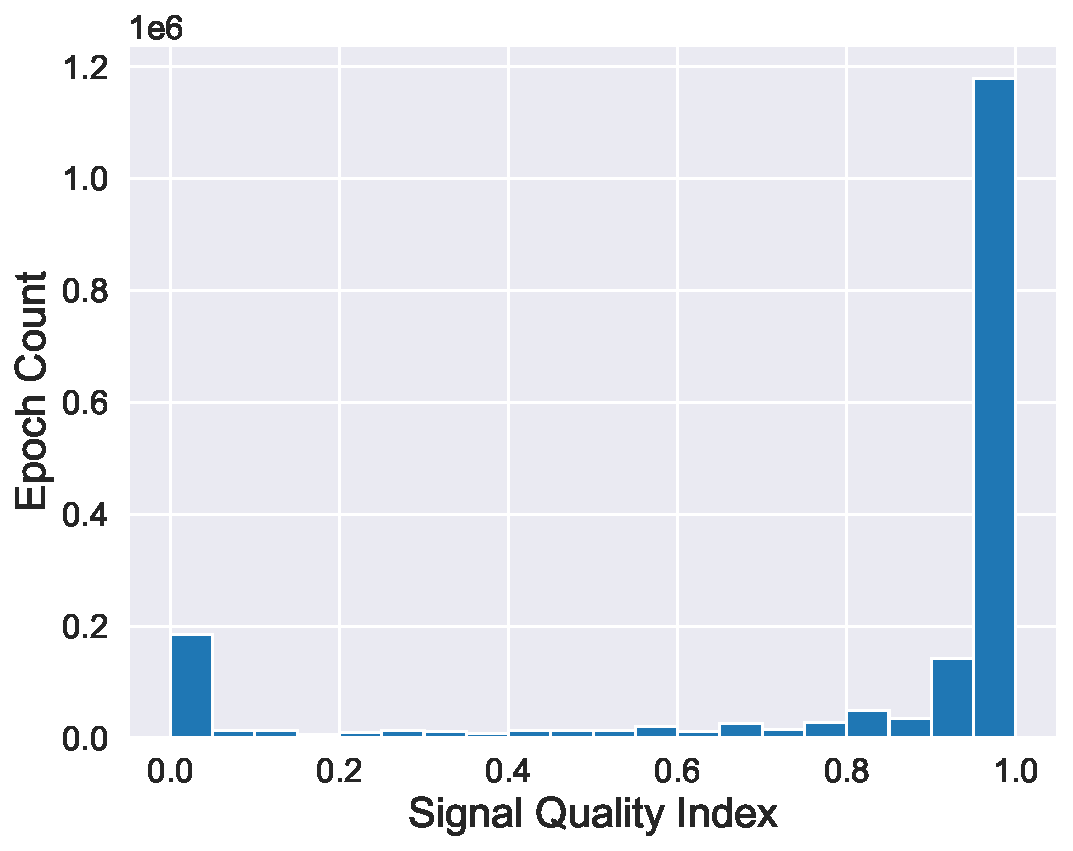
\includegraphics[width=\linewidth]{images/sqi-stats.pdf}
\caption[]{Distribution of SQI for all 5-minute EEG epochs. Consecutive epochs from one EEG recording have a 1-minute gap (hop length).}
\label{fig:sqi-stats}
\end{figure}

As the computation resources and execution time are limited under the circumstances of the Challenge, further offline data selection was conducted according to the signal quality index (SQI). The SQI was computed for every 5-minute epoch as its proportion of ``normal'' 10s segments. A 10s segment is regarded as ``normal'' if no artefact is detected from it, including abnormal values and patterns in the waveform and in the spectrum \footnote{Refer to \url{https://github.com/DeepPSP/cinc2023/utils/artifact_pipeline} for more details.} The distribution of SQI for all 5-minute epochs is collected in Fig. \ref{fig:sqi-stats}. At most one epoch was chosen (SQI $>= 0.95$, or none was chosen) from each recording as a representative of it for developing our neural network models. A total number of xxx (to write) 5-minute epochs were selected.


\subsection{Preprocessing Criteria}
\label{subsec:data_preproc}
% NOT finished

In this subsection, we describe our preprocessing pipeline for model development and making inferences.

The EEG recordings provided by the ICARE dataset have varying numbers of channels (19 - 21) but share a common set of 19 channels. The voltage values of each EEG signal are relative to an ``unknown'' reference potential. Hence in order to align these voltage values, the varying-dimensional EEG signals were transformed into the bipolar format with the following 18 channels
\begin{indentedquote}{0.3in}
\it Fp1-F7, F7-T3, T3-T5, T5-O1, Fp2-F8, F8-T4, T4-T6, T6-O2, Fp1-F3, F3-C3, C3-P3, P3-O1, Fp2-F4, F4-C4, C4-P4, P4-O2, Fz-Cz, Cz-Pz
\end{indentedquote}
18 was chosen since it is the smallest number of bipolar channels to reconstruct the original 19-channel EEG signal.

Bipolar EEGs were further standardized with the following 3 sequential operations:
\begin{itemize}
    \item Butterworth bandpass filter of order 4 and cutoff frequencies 0.5 - 30 Hz;
    \item resample to 100 Hz using polyphase filtering;
    \item rescale to zero mean and unit variance.
\end{itemize}


\subsection{Models and Training Strategies}
\label{subsec:models}
% NOT finished

Considering that there's a clear and widely accepted (also adopted in the Challenge) mapping from CPC values to clinical outcomes as follows:
\begin{itemize}
    \item ``Good outcome'' for CPC $\in \{1, 2\};$
    \item ``Bood outcome'' for CPC $\in \{3, 4, 5\},$
\end{itemize}
and that the CPC values are discrete, we regard the problem as one 5-class classification problem, namely predicting the 5 discrete CPC values.

xxx

The asymetric loss \cite{ridnik2021asymmetric_loss} is
